
\documentclass[a4paper, 10pt]{IEEEconf}  

\usepackage{geometry}
\geometry{a4paper, margin=1in}
    
\usepackage{verbatim}
\usepackage{graphicx}
\usepackage{pdfpages}
\usepackage{cite}
\usepackage{listings}
\usepackage{float}
\usepackage{url}
\usepackage{hyperref}
\usepackage{fancyhdr}

\lstset{
	tabsize=2,
	breaklines=true
}

\setlength{\parskip}{1em}
\onecolumn

\title{\LARGE \bf Project 1: Pneumatic Cylinder\\Mechatronics  282 778}
\author{Marc Alexander Sferrazza \\ 12164165
\thanks{This work was not supported by any organization}
\thanks{Faculty of Mechatronics Engineering, Massey University, Albany, Auckland, New Zealand
        {\tt\small Progress of project: https://github.com/alex1v1a/Mechatrnoics/} } }

\begin{document}

\maketitle

%\begin{figure}[H]
%  \includegraphics[width=\linewidth]{images/final}
%  \label{fig:Final Product}
%\end{figure}

\thispagestyle{empty}
\pagestyle{plain}


%%%%%%%%%%%%%%%%%%%%%%%%%%%%%%%%%%%%%%%%%%%%%%%%%%%%%%%%%%%%%%%%%%%%%%%%%%%%%%%%

\begin{abstract}

Pneumatic actuation controlled project involving the projection of tennis balls. The projectiles are deployed from the actuation controlled device at fixed intervals and have an optional override to deploy manually. 
\\

The project involves constructing a frame in which will enclose and secure all parts in an orderly safe fashion; designing and building the PCB circuit with the consideration of controlling the solenoid, reading and displaying the extension of the actuator.
\\

In this process, acquired Mechatronics skills are tested to build a devices which has mechanical, electrical and programming components with consideration of materials properties. To utilise all of the skills on a basic level of which can measure the performance and aptitude of converging these skills, and how things are done individually. While there are many methods to preform the task, consisting of different professional approaches is key for performance on an industry level.

\end{abstract}


\clearpage
\tableofcontents
\listoffigures
%\listoftables
\thispagestyle{empty}
\clearpage
\twocolumn

%%%%%%%%%%%%%%%%%%%%%%%%%%%%%%%%%%%%%%%%%%%%%%%%%%%%%%%%%%%%%%%%%%%%%%%%%%%%%%%%
%%%%%%%%%%%%%%%%%%%%%%%%%%%%%%%%%%%%%%%%%%%%%%%%%%%%%%%%%%%%%%%%%%%%%%%%%%%%%%%%

\setcounter{page}{1}

\section{INTRODUCTION}

The project is to utilise skills acquired, to build a mechatronic device that uses an actuation and sensing sub-system, with a control interface to time the interval in which it takes to deploy a projectile (tennis ball) from the hopper. The hopper can hold up to 3 projectiles (tennis balls) which are pre-loaded, and will deploy with a fixed time interval or manual override ejection.

%%%%%%%%%%%%%%%%%%%%%%%%%%%%%%%%%%%%%%%%%%%%%%%%%%%%%%%%%%%%%%%%%%%%%%%%%%%%%%%%

\subsection{Aims \& Objectives}

To build a mechatronic sub-system device, integrating actuation, sensing, and control sub-systems.

The key objectives to cover in this task includes

\begin{itemize}
	\item Control the extension and contraction of a pneumatic cylinder.
	\item Measure the extension and contraction of a pneumatic cylinder.
	\item Integrate the mechatronic actuation, sensor, and control sub-systems in order to eject projectiles from a hopper with a fixed time period between deployments.
\end{itemize}

There are no constraints at which the design is to be achieved, leaving the best found method determined by the development. Therefore the process and development in the design is open for opinion given appropriate reasoning.

%%%%%%%%%%%%%%%%%%%%%%%%%%%%%%%%%%%%%%%%%%%%%%%%%%%%%%%%%%%%%%%%%%%%%%%%%%%%%%%%
%%%%%%%%%%%%%%%%%%%%%%%%%%%%%%%%%%%%%%%%%%%%%%%%%%%%%%%%%%%%%%%%%%%%%%%%%%%%%%%%

\section{METHOD}

Detailed description of what was done, how, and why. 
***********************

%%%%%%%%%%%%%%%%%%%%%%%%%%%%%%%%%%%%%%%%%%%%%%%%%%%%%%%%%%%%%%%%%%%%%%%%%%%%%%%%

\subsection{Frame Material Selection}

Planning in design for structural integrity is subject to the workspaces constraints, while there are many methods of which the design can be achieved, in a long life usage of the project using metals can prove effective; however in the projects scope the projectiles may be launched a minimum of eight times effectively without damage to the chassis. Therefore the design materials are chosen subject to a prototype friendly, cost effective method which will meet the required eight successful launches for demonstration and any additional deployment during testing and compensation of the demonstration. 

The estimated reasonable number of ejections required used is 100 cycles of both extension and contraction for the pneumatic cylinder, as this is the highest action point of the device, while all other parts remain fixed except the projectiles themselves. With considerations of this, and analysis provided such as FEA strain tests over 200 (double the required) cycles with Solidworks 2015 and the isolated actuation frame the selected material chosen is entirely based on acrylic with the exception of PVC piping (explained further in frame design for the hopper pre-load). 

\begin{figure}[H]
  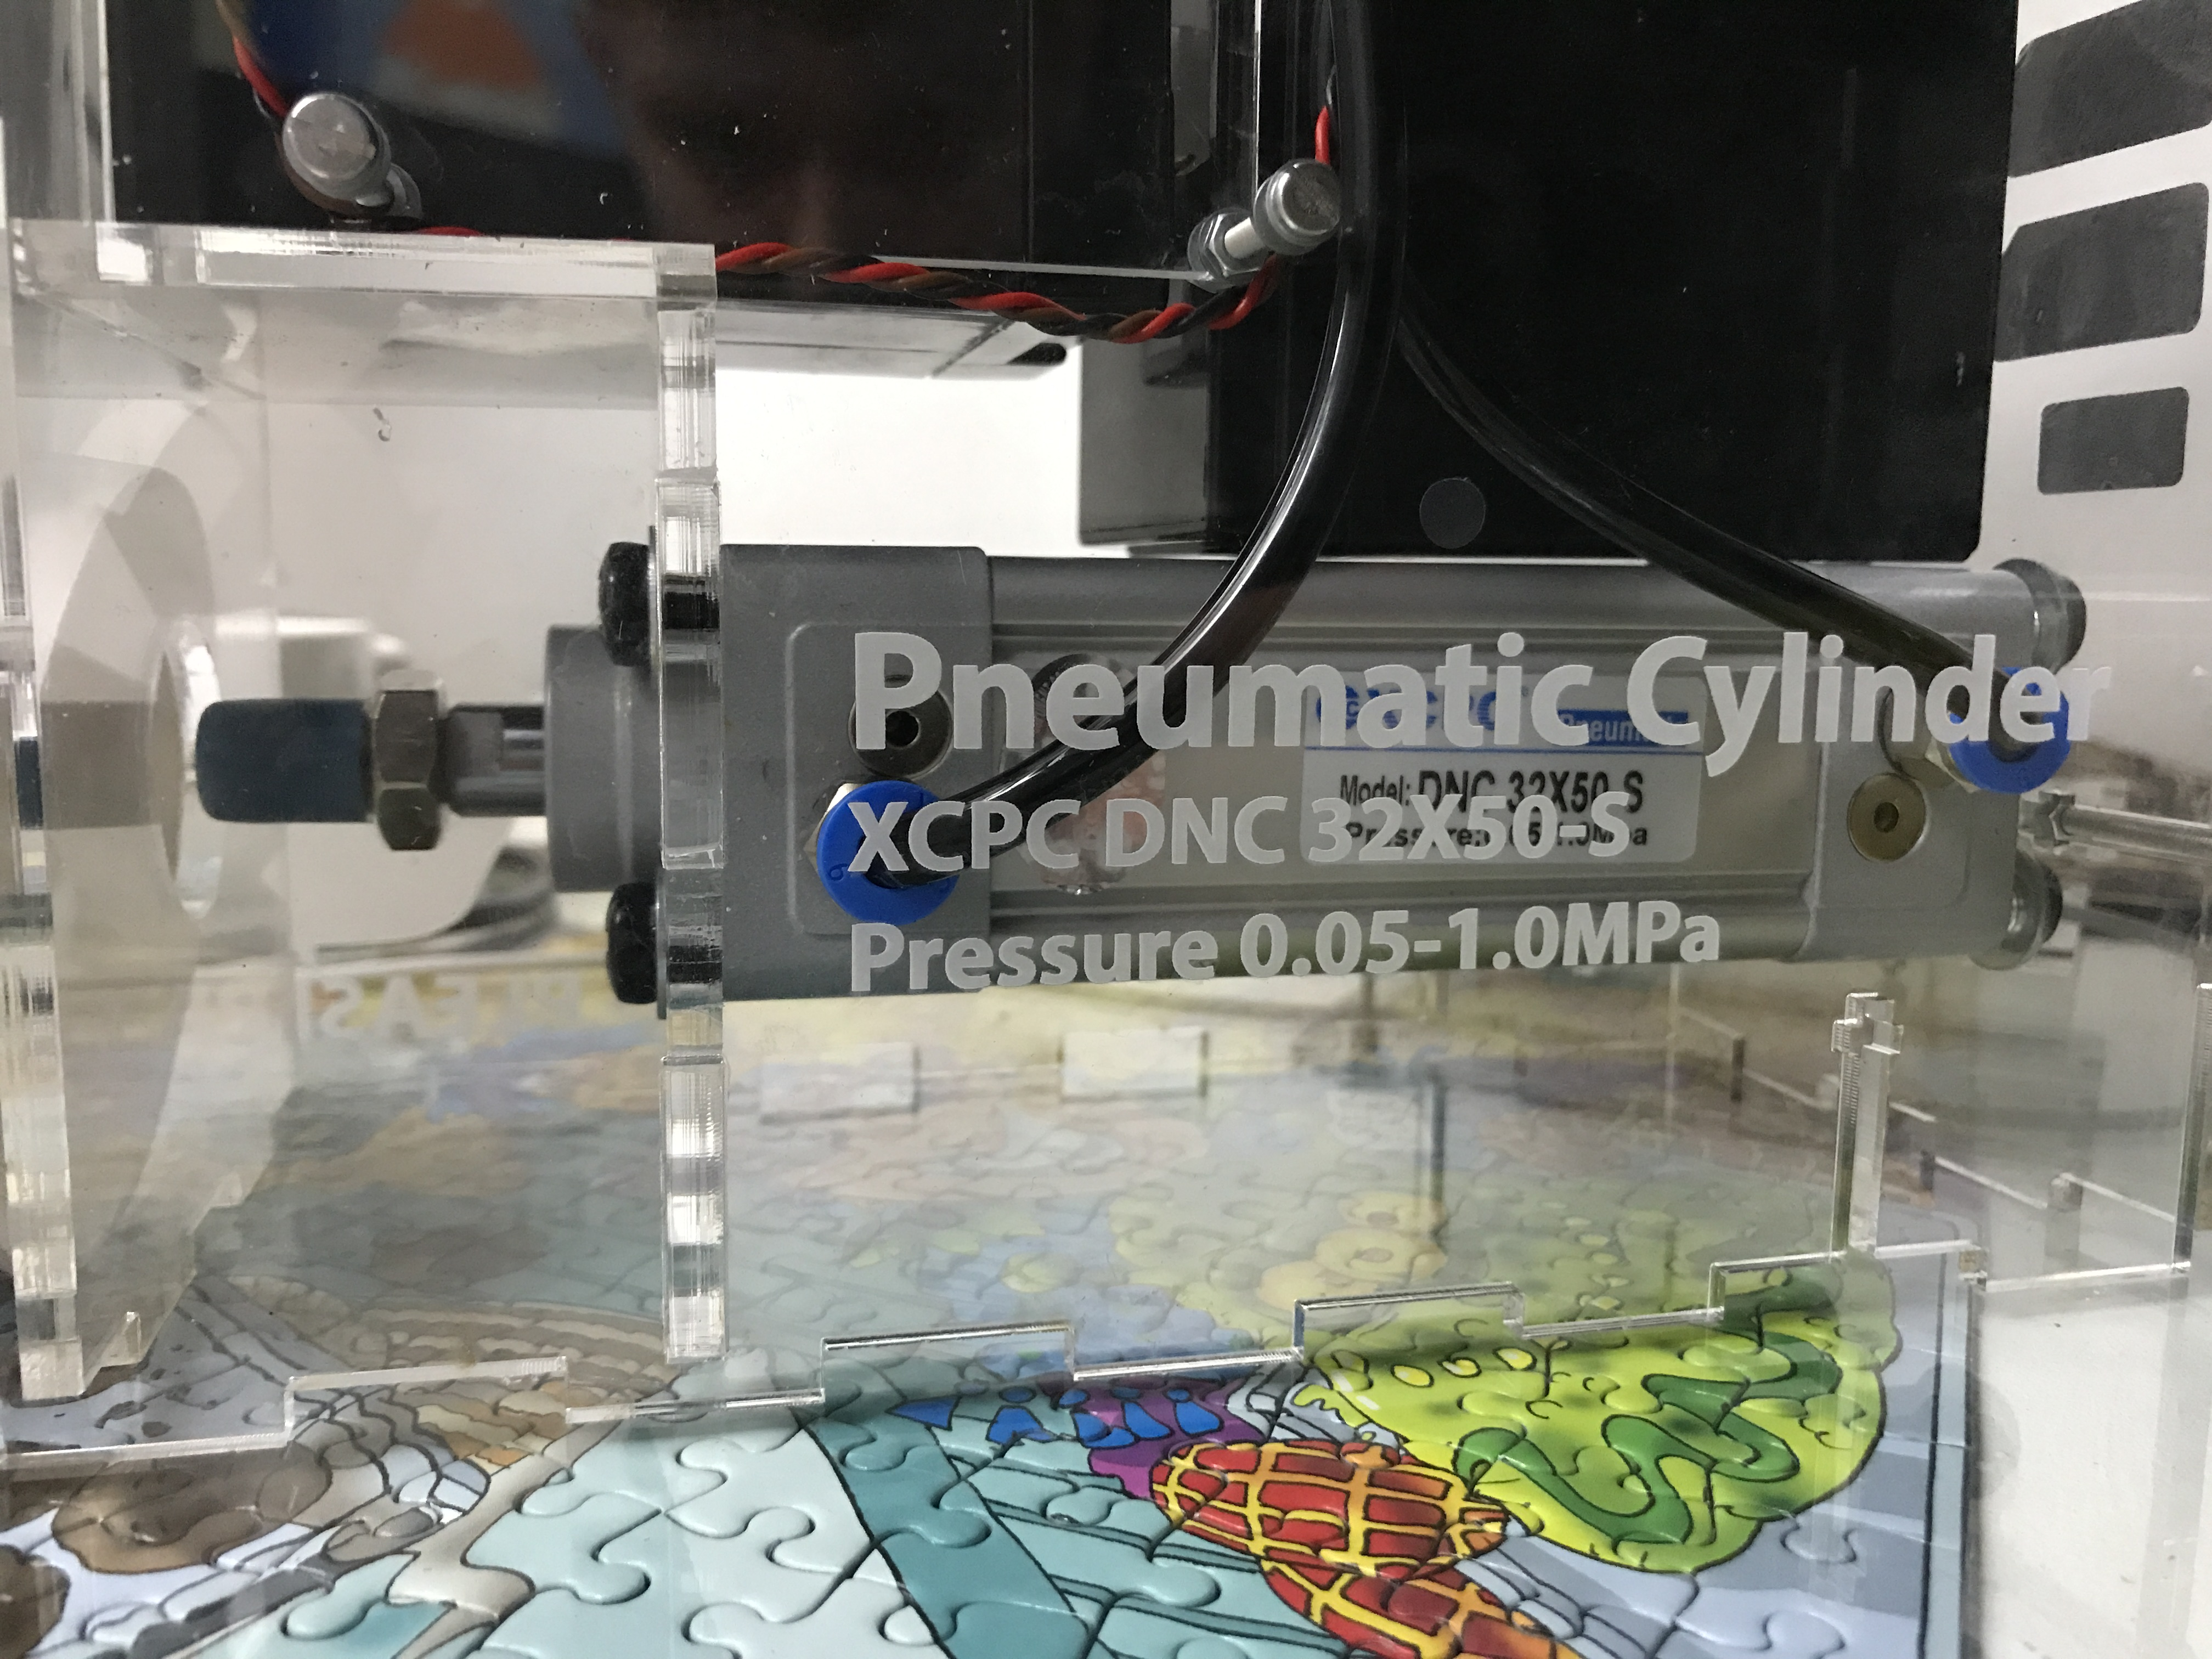
\includegraphics[width=\linewidth]{images/cylinder}
  \caption{Isolated actuation frame}
  \label{fig:Isolated actuation frame}
\end{figure}

While acrylic is more brittle then other ready available materials such as MDF, acrylic has the beneficial key feature of being fully transparent, so a full display of all parts can be monitored, and the full demonstration of all internal parts can be observed. Another key reason for this choice in material is the bonding of surfaces in the respect that with specific chemicals applied the surfaces fuse together and become bonded, almost in the sense they were moulded that way which with correct design can spread force through the entire chassis.


%%%%%%%%%%%%%%%%%%%%%%%%%%%%%%%%%%%%%%%%%%%%%%%%%%%%%%%%%%%%%%%%%%%%%%%%%%%%%%%%

\subsection{Frame design}

PVC pipe for hopper to contain the pre-loaded projectiles and the 
*************

\begin{figure}[H]
  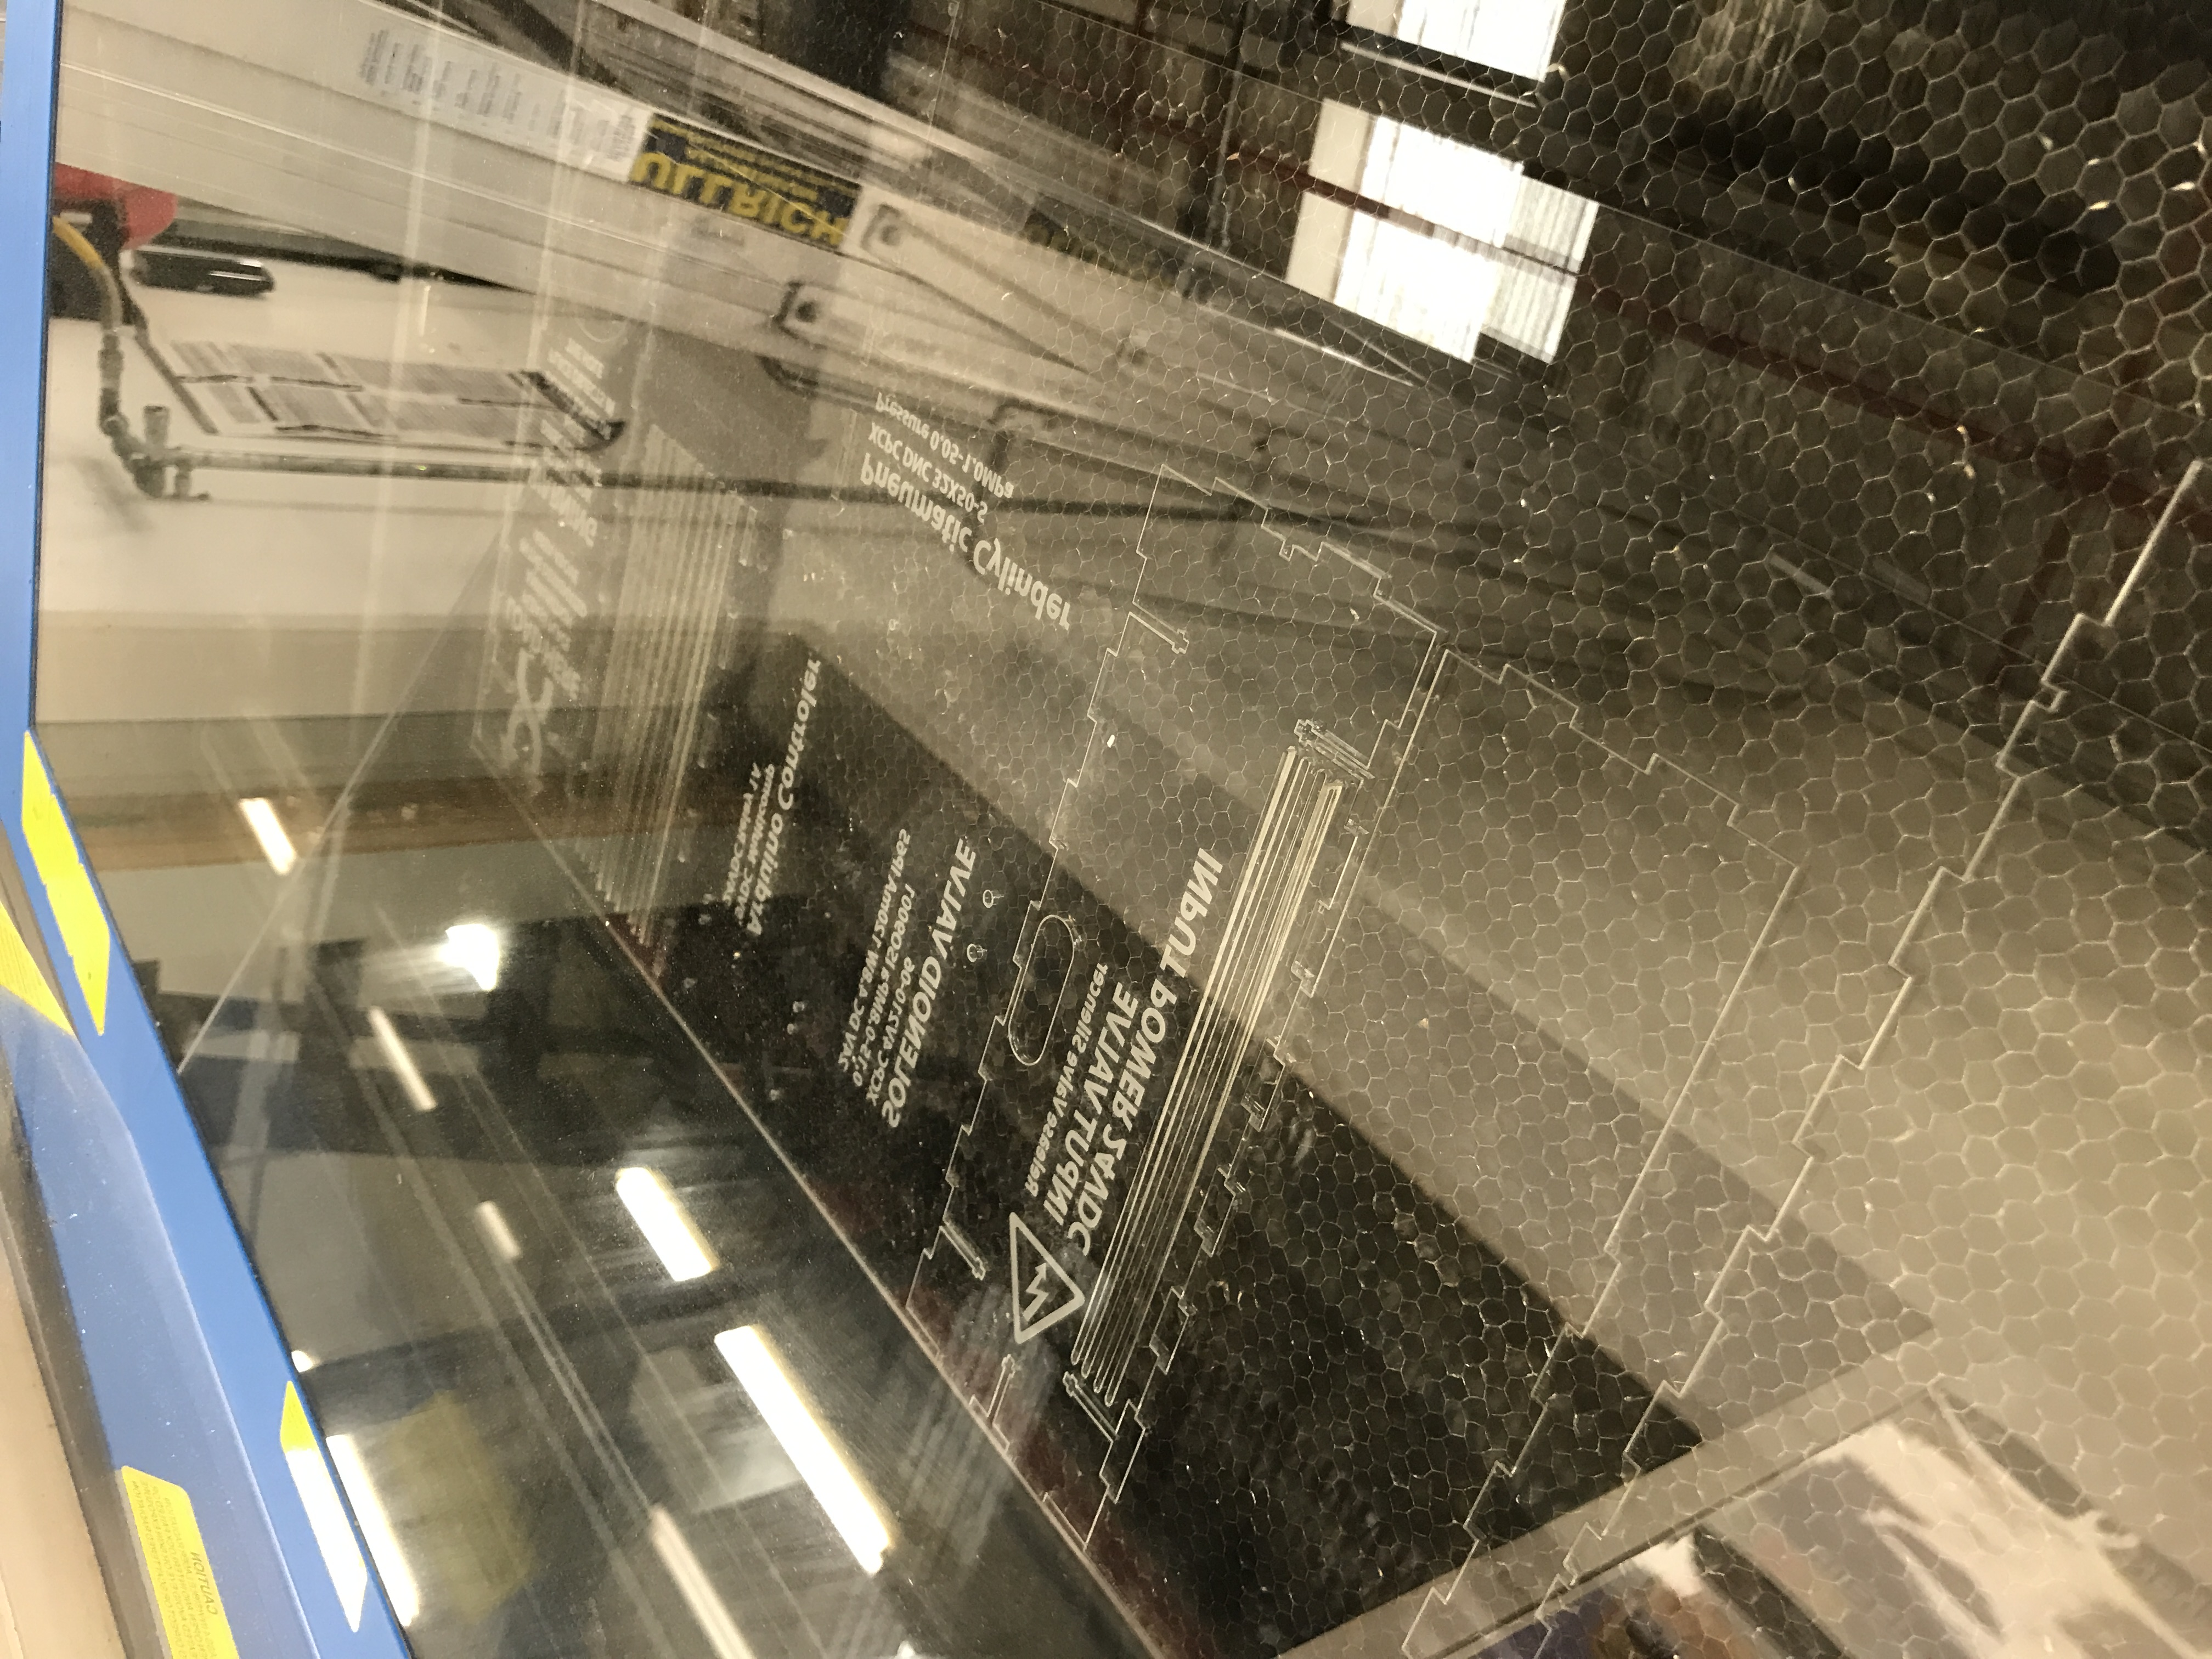
\includegraphics[width=\linewidth]{images/laser}
  \caption{Laser cutting the frame}
  \label{fig:Laser cutting the frame}
\end{figure}


\begin{figure}[H]
  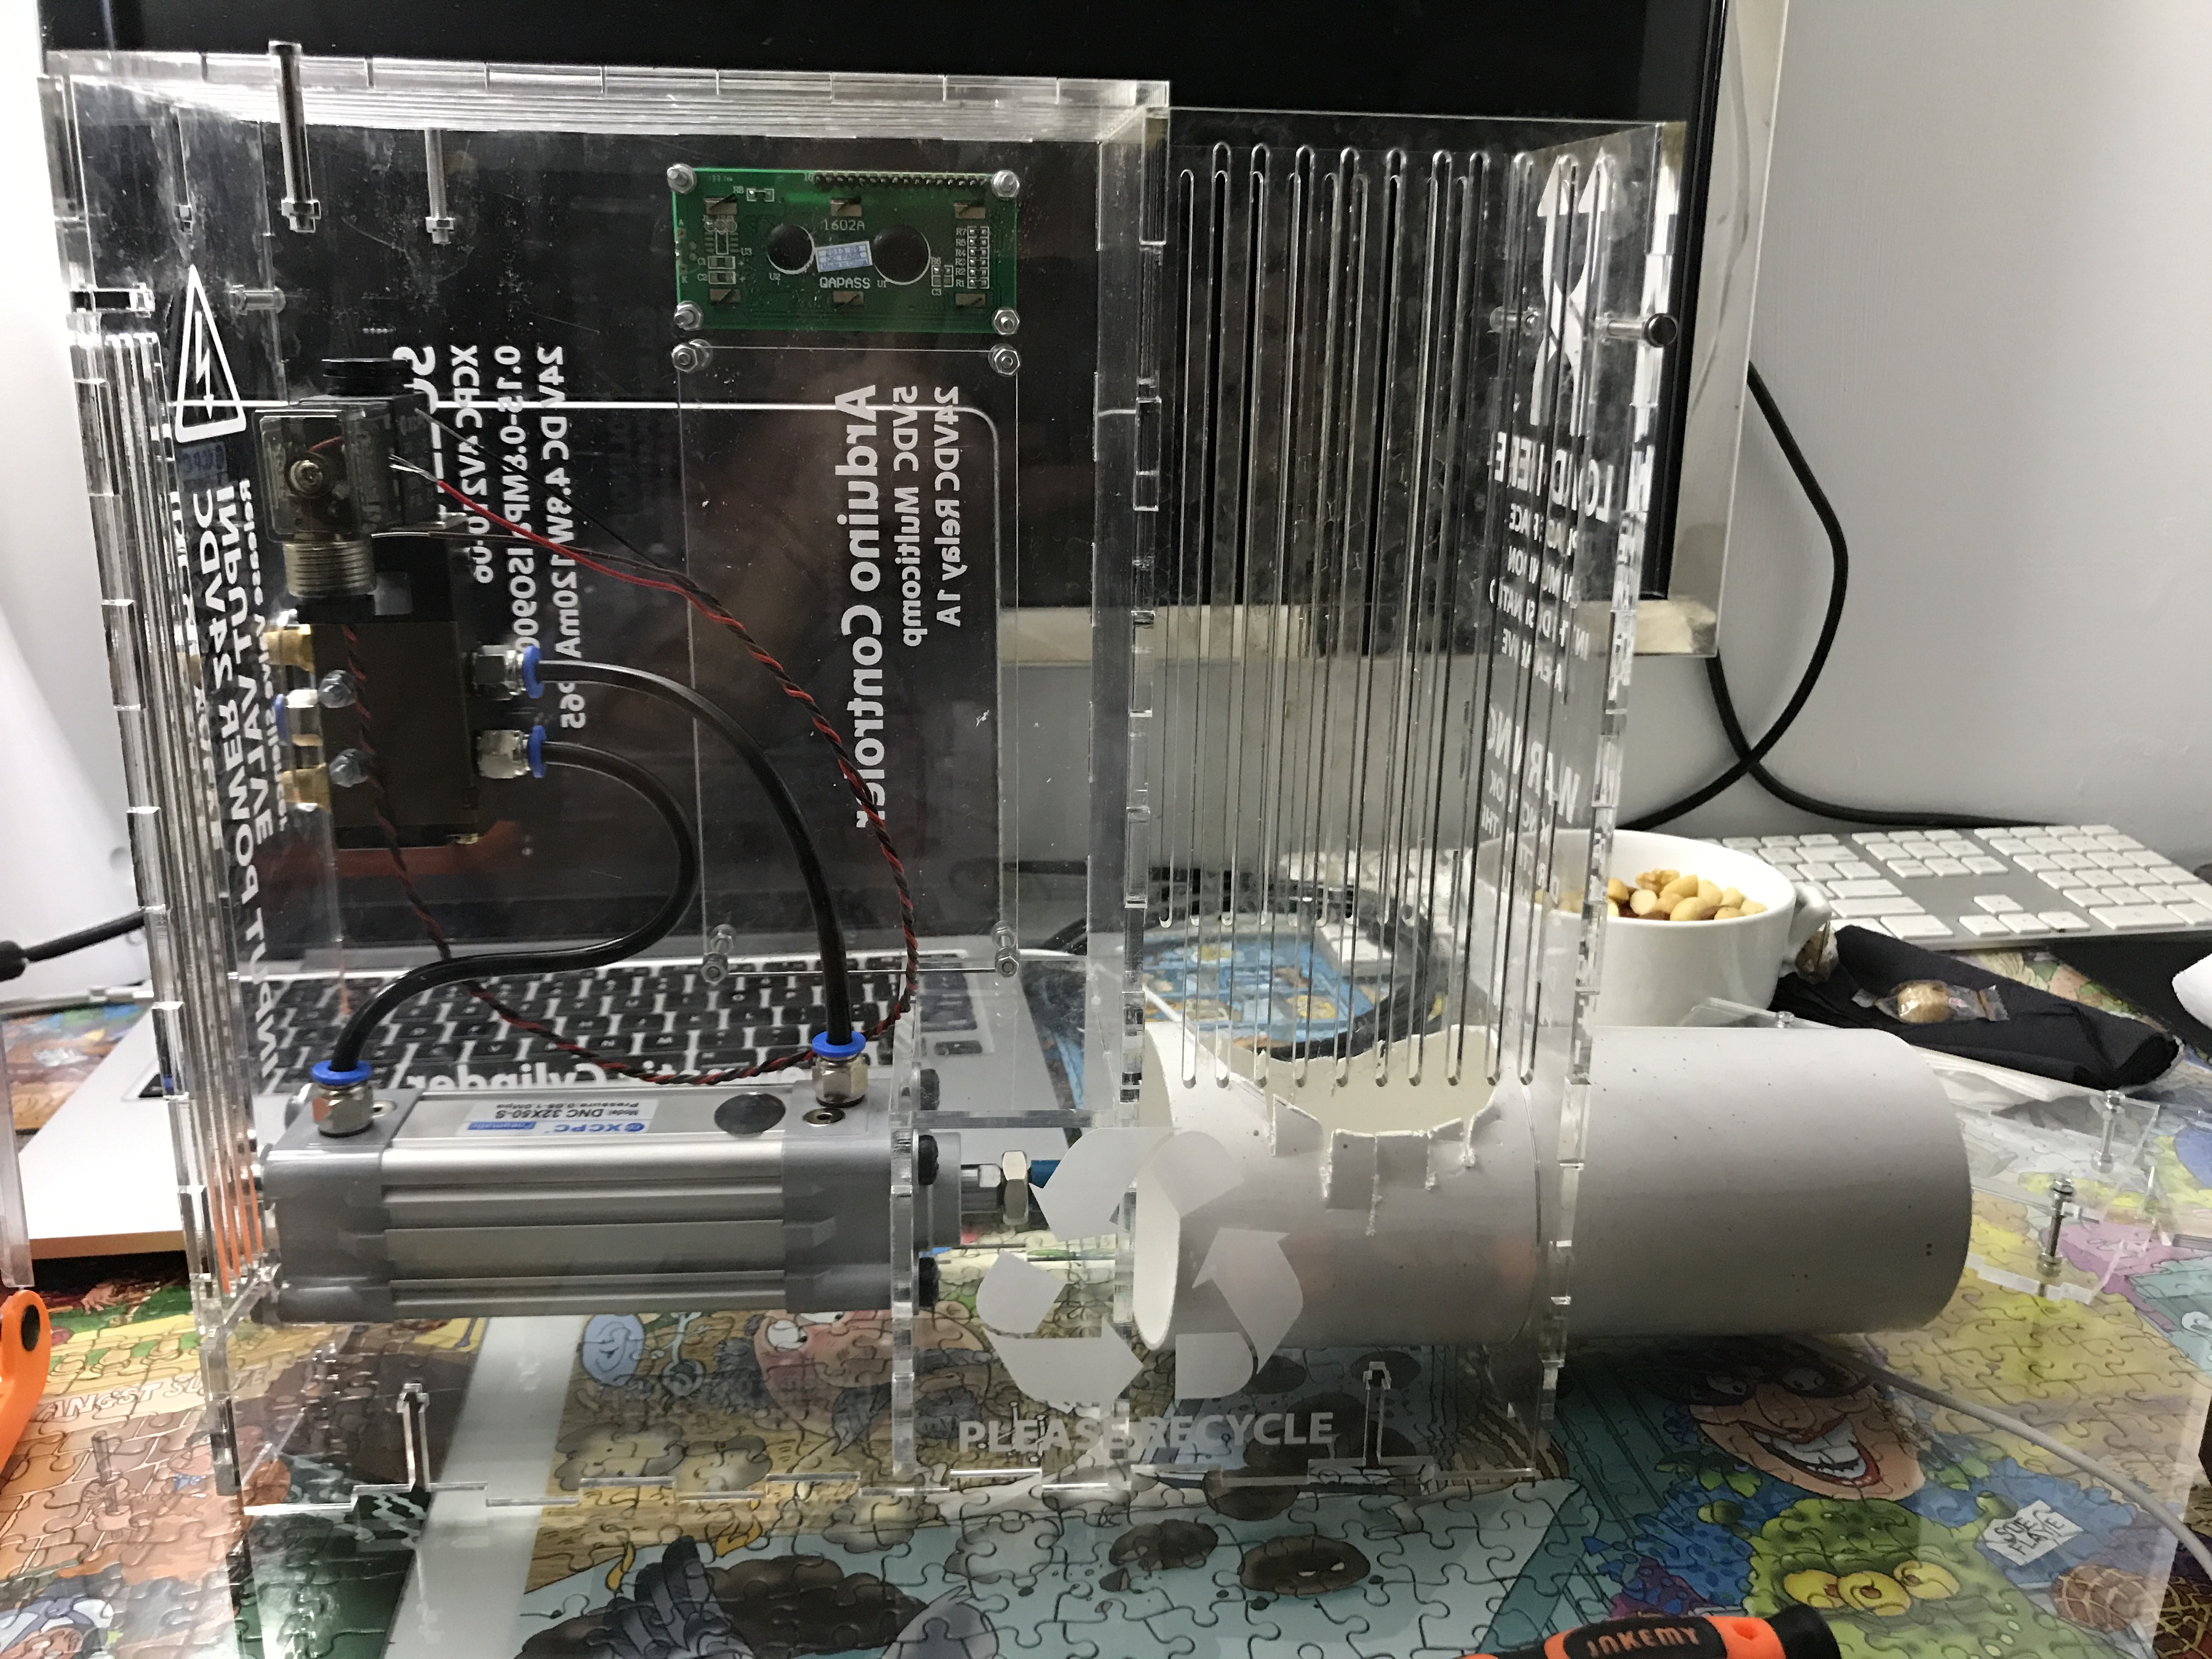
\includegraphics[width=\linewidth]{images/Frame}
  \caption{Basic stripped frame before population}
  \label{fig:Basic stripped frame before population}
\end{figure}

%%%%%%%%%%%%%%%%%%%%%%%%%%%%%%%%%%%%%%%%%%%%%%%%%%%%%%%%%%%%%%%%%%%%%%%%%%%%%%%%

\subsection{Bonding \& Linkages}

To secure the frame M3 30mm bolts and nuts were used with 8xM6 bolts securing the pneumatic actuator. All mounting and fastening of internal components is also achieved with M3 size bolts, while dampening foam has been used to cushion some surfaces.

The primary influence in structure bonding is C105 also known as acrylic weld but not to be mistaken with C502 also known as super glue for plastics and rubbers, which offers a different method of molecular bonding of surfaces. The advantage of C105 is that it is extremely thin comparable with water and preforms quick bonding which results in two or more surfaces being fused like overlaying corrugated iron.

The 105 Acribond contains
\begin{itemize}
	\item U.N. 1593 METHYLENE CHLORIDE CAS No. 75-09-2
	\item U.N. 1710 TRICHLOROETHYLENE STABILIZED CAS No. 79-01-6
	\item U.N. 1247 METHYL METHACRYLATE MONOMER CAS No. 80-62-6
\end{itemize}
PG III, HAZCHEM CODE 2Z, Class 6.1

For a more in depth discussion on bonding materials and useful chemistry for plastics and rubbers ePlastics website is linked in the reference section \cite{ePlastic}; the 105 Acribond link \cite{105} is also provided.

%%%%%%%%%%%%%%%%%%%%%%%%%%%%%%%%%%%%%%%%%%%%%%%%%%%%%%%%%%%%%%%%%%%%%%%%%%%%%%%%

\subsection{Power Supply}

The available option of a 24VDC bench power supply is provided, however for ease of use in testing and probability an internal power supply has been integrated. The selected cells are 2x 12VDC 7AH Gel AGM SLA batteries connected in series to provide a stable constant reliable power source which does not require frequent charging. The resultant supply is 24VDC 7AH for reference. 

There is a built in universal charge port using banana sockets of which any appropriate SLA 24V charger can be used. Due to the nature of the batteries and the self maintenance hydrogen gas released the frame includes vents for any build up of gas or excess heat from components.

\begin{figure}[H]
  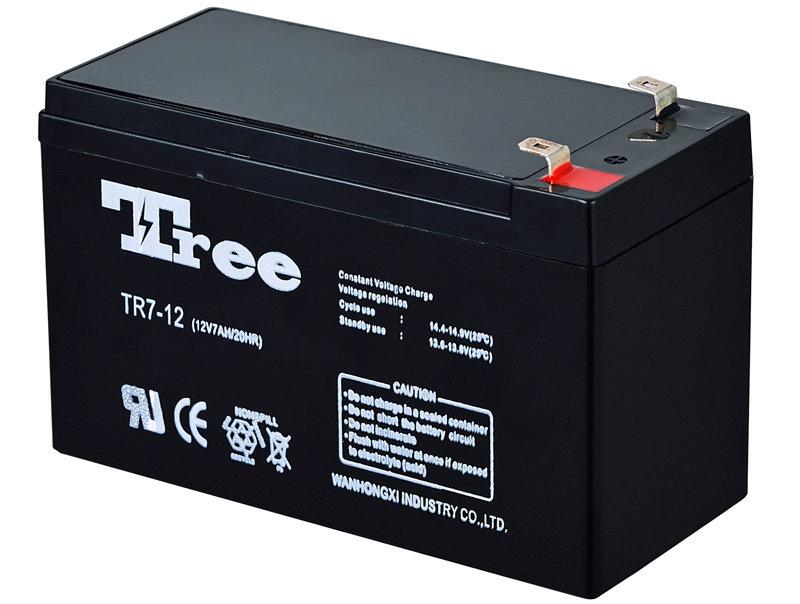
\includegraphics[width=\linewidth]{images/Battery}
  \caption{Tree Battery 12VDC 7AH Gel AGM SLA}
  \label{fig:Basic stripped frame before population}
\end{figure}

%%%%%%%%%%%%%%%%%%%%%%%%%%%%%%%%%%%%%%%%%%%%%%%%%%%%%%%%%%%%%%%%%%%%%%%%%%%%%%%%

\subsection{Eagle PCB}

Using Eagle CAD-soft from Autodesk \cite{eagle} a PCB is designed and implimented. 

The PCB design includes the following
\begin{itemize}
	\item Arduino controller
	\item Voltage regulator (24VDC to 5VDC)
	\item Relay from the Arduino to the solenoid (5VDC to 24VDC/120VDC 1A)
	\item Relevant LED's
	\item Safety features e.g. fuses (0.5A)
	\item Ground Core
\end{itemize}

The components are shown in a working order below. The LED's indicate the state of each action, with the red LED relating to power from the source at each stage 24VDC. Yellow being the state of the stage after some processing, the first being the regulation from 24VDC to 5VDC, the second being the normally closed side of the relay or contraction of the actuation arm. Finally the green LED is for the extension state of the actuation arm. These LED's are for status states only and debugging thus why they are not mounted and displayed on the enclosure although visible.

\begin{figure}[H]
  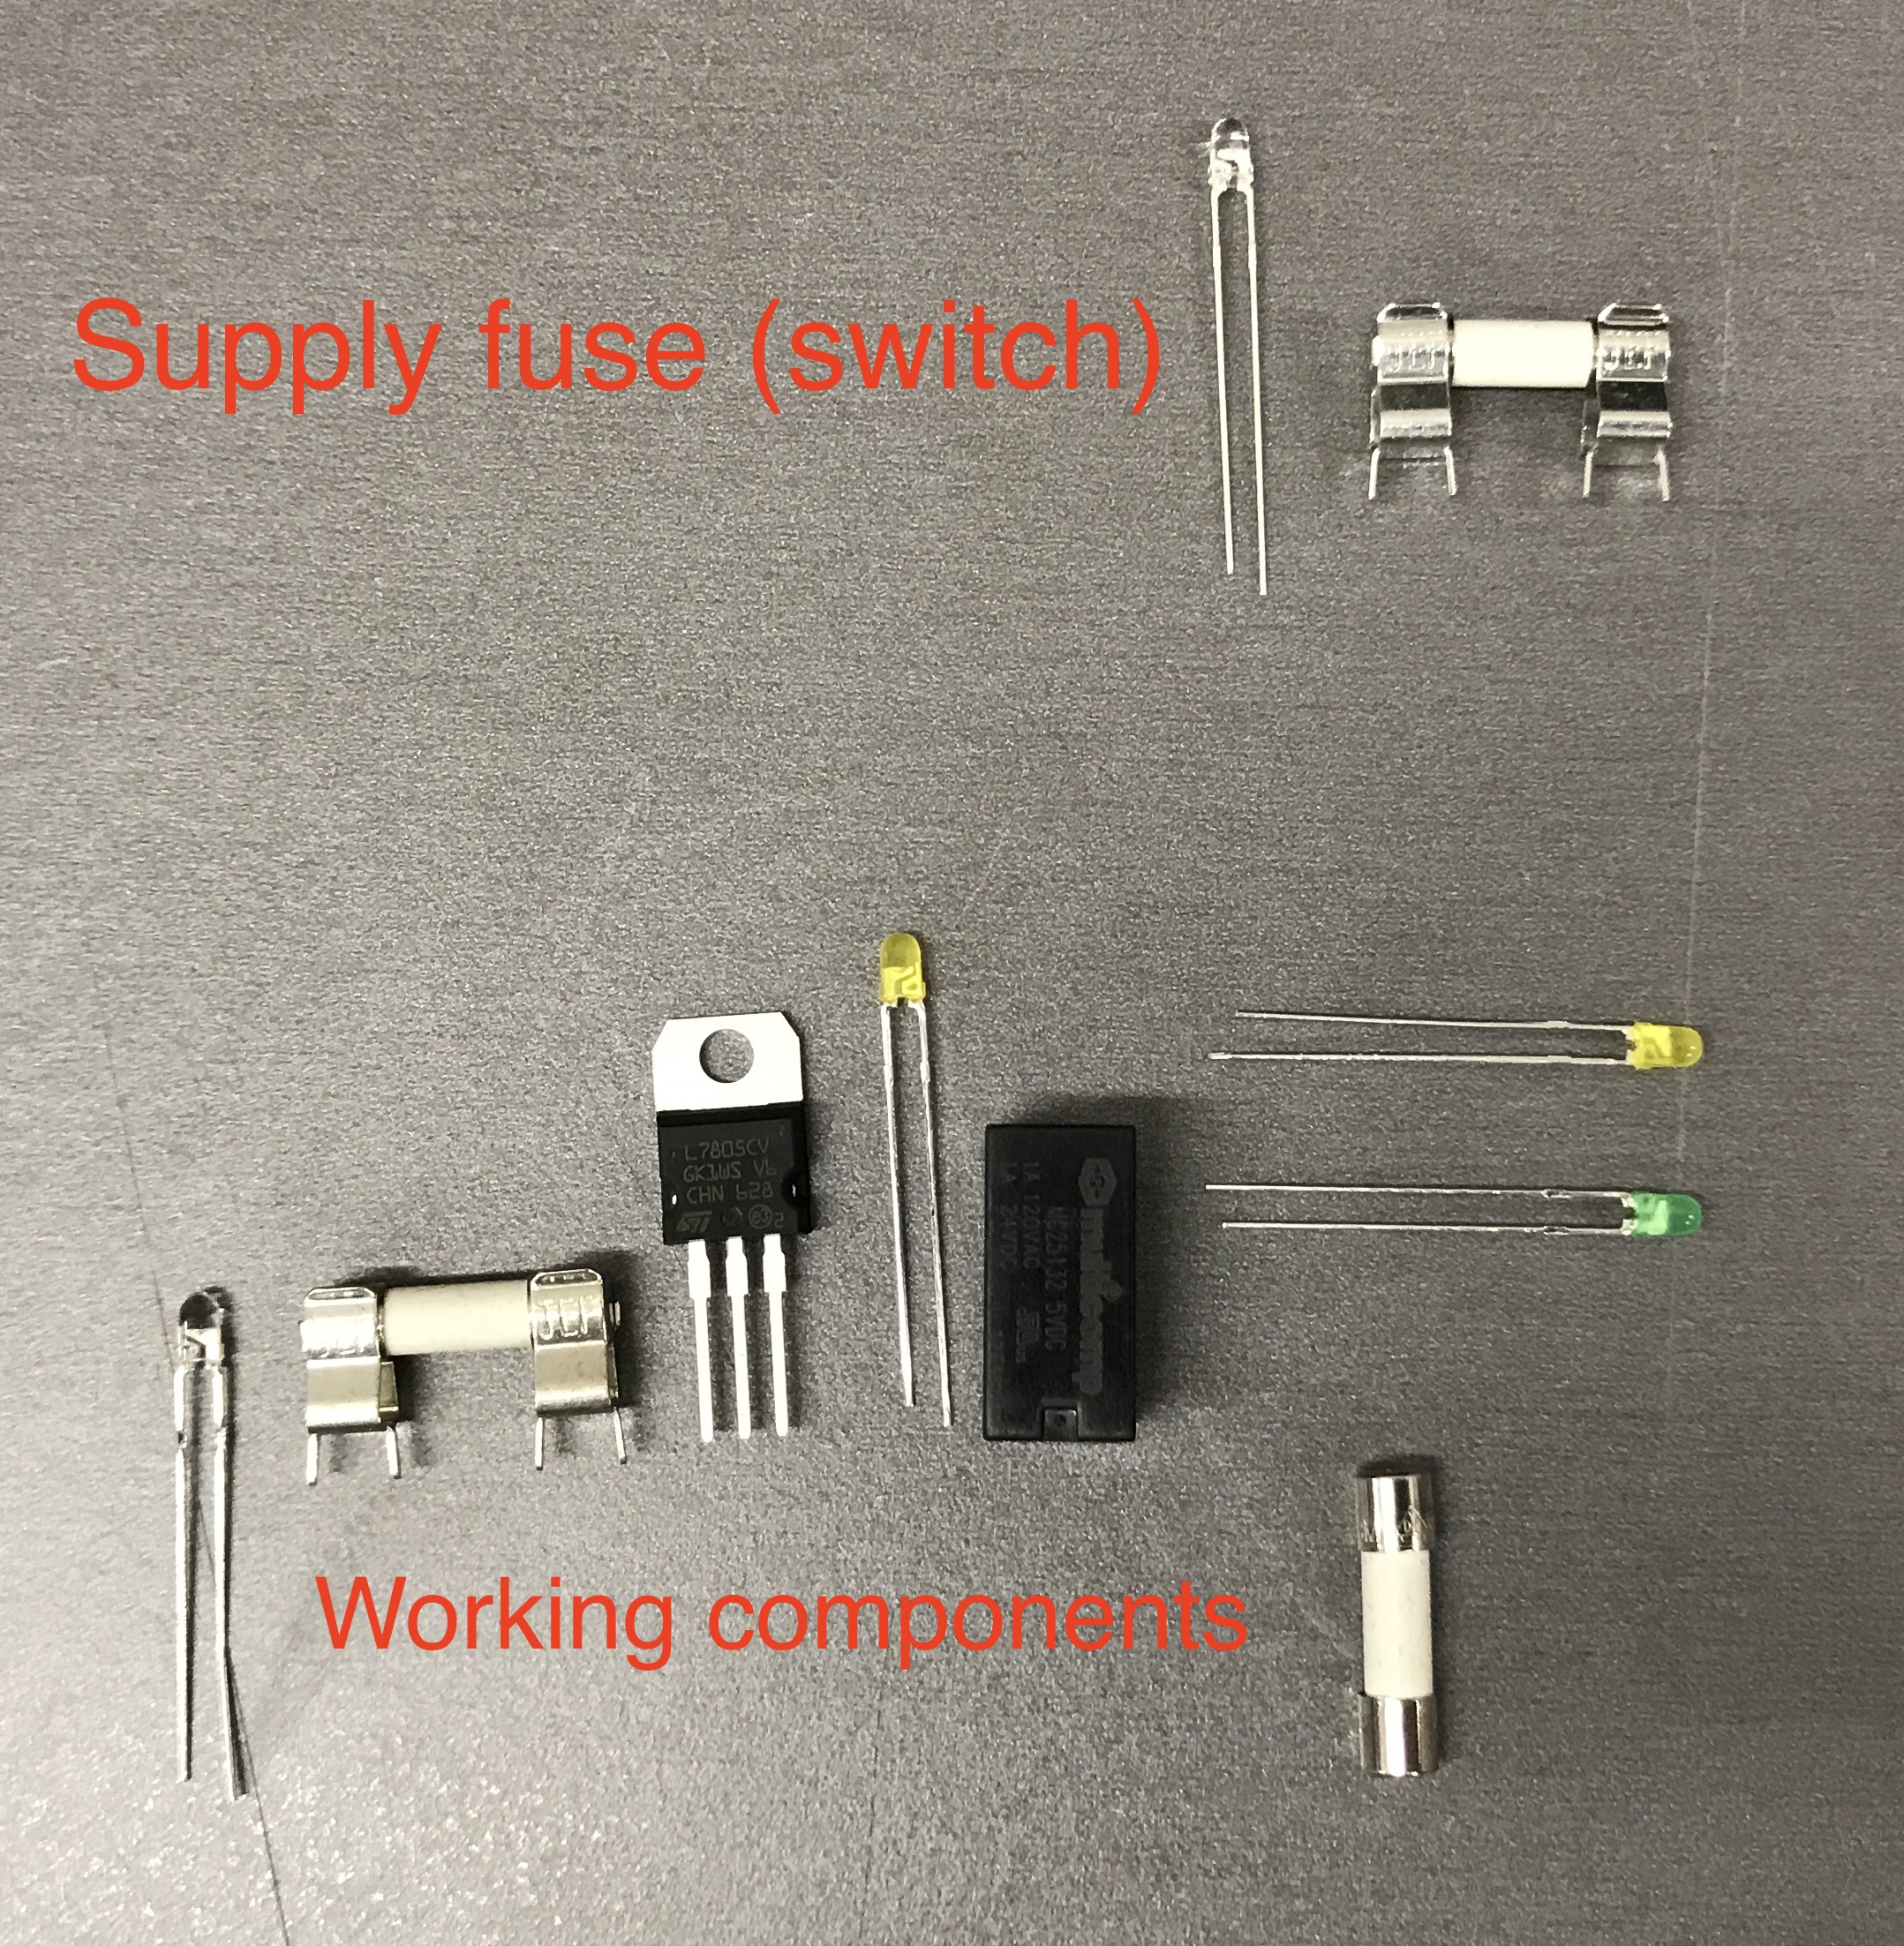
\includegraphics[width=\linewidth]{images/parts}
  \caption{Components of design}
  \label{fig:Components of design}
\end{figure}

A schematic of the design is given below. The design does not include capacitors after the regulator (or an attached heatsink) due to the current draw being less the 20\% of the capacity of the transistor which is 1A and is not required.

\begin{figure}[H]
  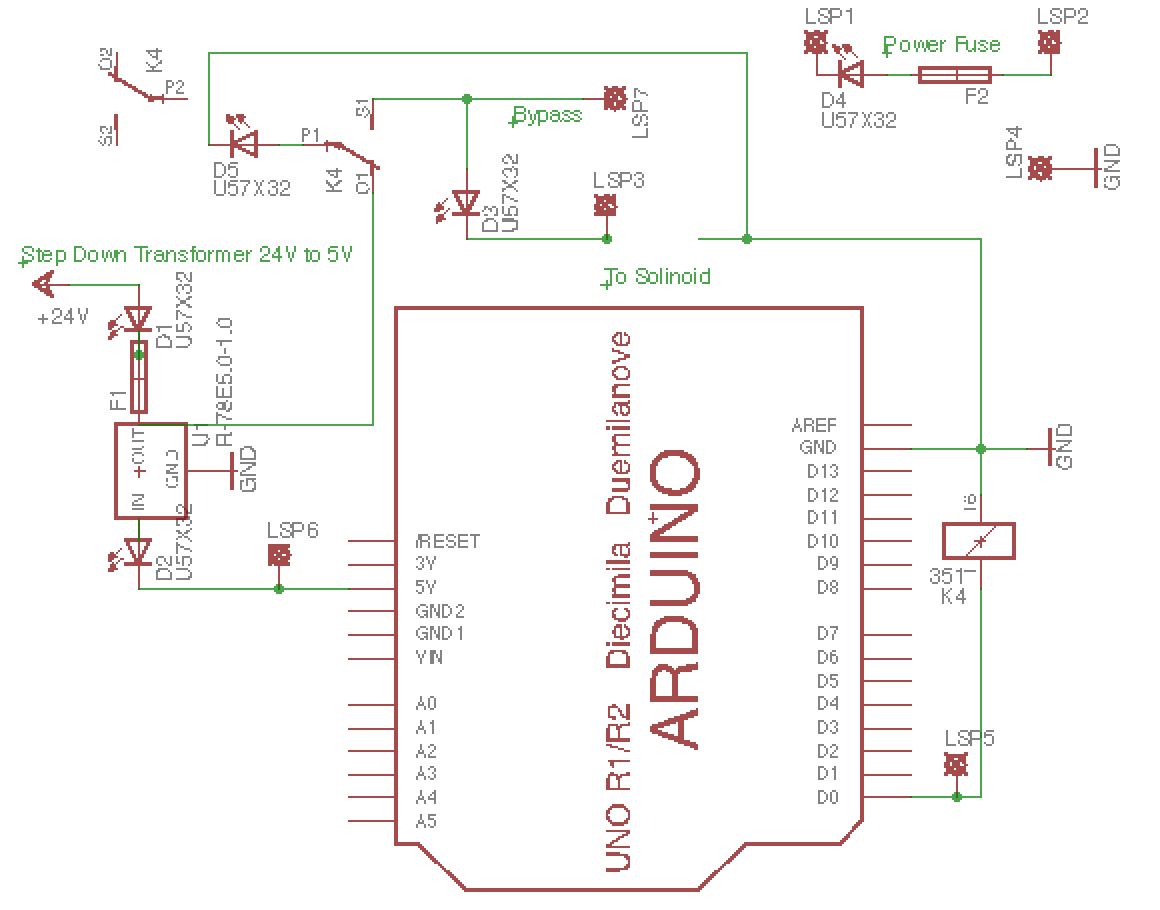
\includegraphics[width=\linewidth]{images/Schematic}
  \caption{Schematic}
  \label{fig:Schematic}
\end{figure}

The board drill out design is shown below. The purpose of this layout being a seperate entity rather then a shield of the Arduino, this is for display purposes only, and to preform visual inspection from the exterior of the enclosure for assessment and debugging. 

\begin{figure}[H]
  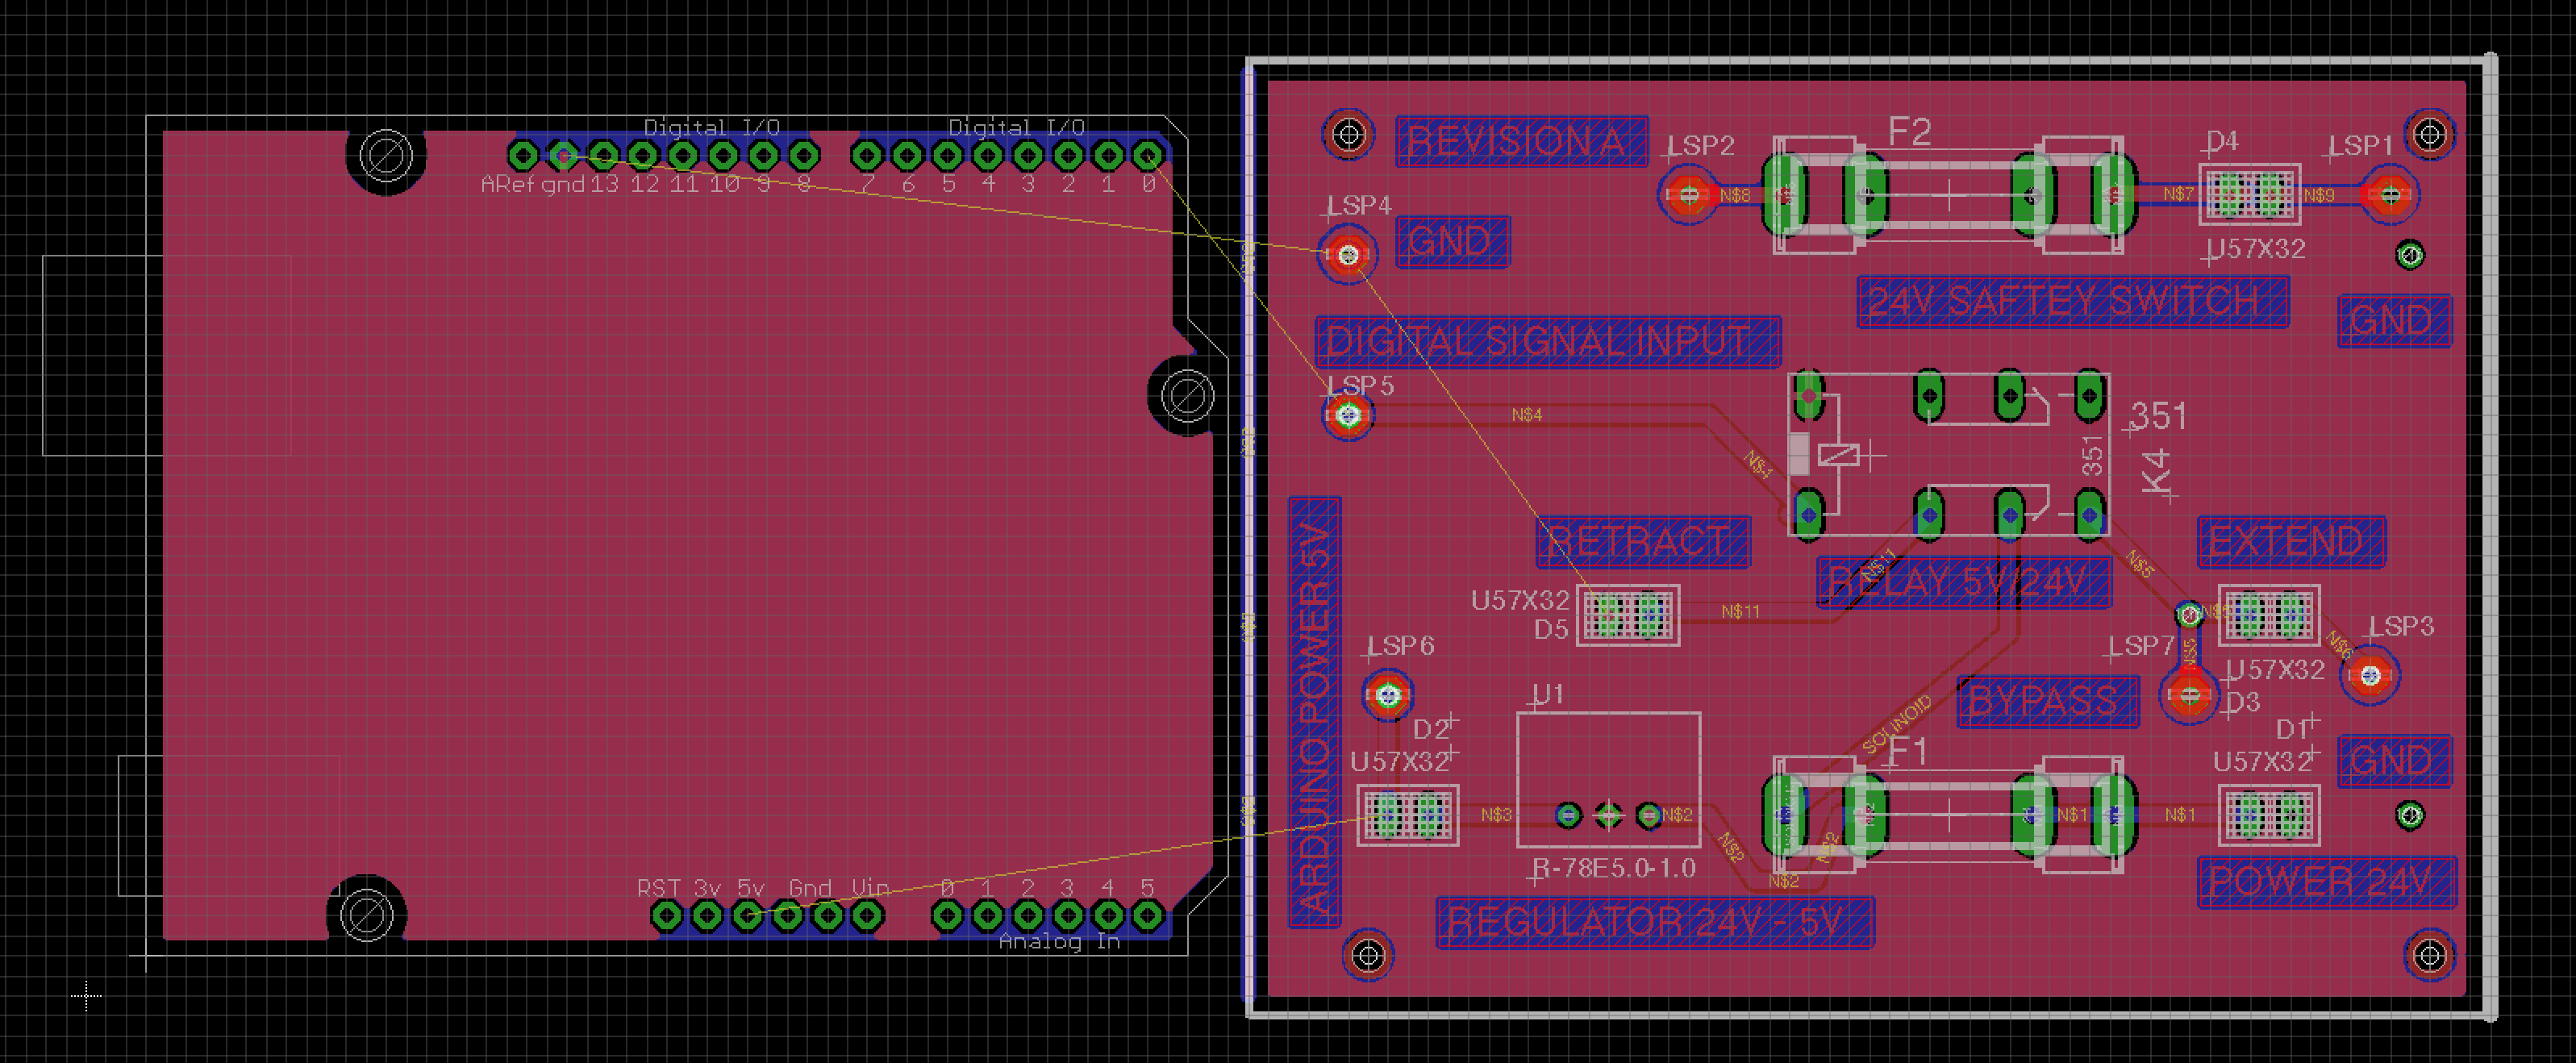
\includegraphics[width=\linewidth]{images/Board}
  \caption{Board design}
  \label{fig:Board design}
\end{figure}

%%%%%%%%%%%%%%%%%%%%%%%%%%%%%%%%%%%%%%%%%%%%%%%%%%%%%%%%%%%%%%%%%%%%%%%%%%%%%%%%

\subsection{Sensor Selection}

In order to measure the distance of the pneumatic actuation arm a form of sensor is acquired. The sensor chosen is the *****, this was selected due to the *********** and the linear properties of the sensors measurement, without issues from depreciation due to limited cycles.

The Actuation is measured with the ******** sensor and sent to the Arduino, which in turn translates the read value from voltage to decimal and is displayed in millimetres on the mounted LCD display located above the Arduino and PCB on the inside of the enclosure. 

%\begin{figure}[H]
%  \includegraphics[width=\linewidth]{images/sensor}
%  \caption{Selected sensor}
%  \label{fig:Selected sensor}
%\end{figure}

%%%%%%%%%%%%%%%%%%%%%%%%%%%%%%%%%%%%%%%%%%%%%%%%%%%%%%%%%%%%%%%%%%%%%%%%%%%%%%%%

\subsection{Programming}

The selected device for use as the controller, and to measure and display the extension is the Arduino Uno. The reasons this was the selected micro-controller board is for no other then being cost effective, as this was taken from past years projects. As there were no specifications on what must be used this was the most appropriate solution.

A summary of the code is shown in the appendix which covers in full the method of deploying the projectiles, the override function, and displaying the displacement of the actuator. Please see the comments embedded in the code for a more step by step detailed explanation for what is being processed.

%%%%%%%%%%%%%%%%%%%%%%%%%%%%%%%%%%%%%%%%%%%%%%%%%%%%%%%%%%%%%%%%%%%%%%%%%%%%%%%%
%%%%%%%%%%%%%%%%%%%%%%%%%%%%%%%%%%%%%%%%%%%%%%%%%%%%%%%%%%%%%%%%%%%%%%%%%%%%%%%%

\section{RESULTS}



%\begin{figure}[H]
%  \includegraphics[width=\linewidth]{images/final}
%  \caption{The final product}
%  \label{fig:The final product}
%\end{figure}

%\begin{figure}[H]
%  \includegraphics[width=\linewidth]{images/final2}
%  \caption{The final product side 2}
%  \label{fig:The final product side 2}
%\end{figure}

%%%%%%%%%%%%%%%%%%%%%%%%%%%%%%%%%%%%%%%%%%%%%%%%%%%%%%%%%%%%%%%%%%%%%%%%%%%%%%%%
%%%%%%%%%%%%%%%%%%%%%%%%%%%%%%%%%%%%%%%%%%%%%%%%%%%%%%%%%%%%%%%%%%%%%%%%%%%%%%%%

\section{OUTCOMES}

Successfully achieved and built a mechatronic sub-system using the following

\begin{itemize}
	\item Sensing elements and signal conditioning used within a mechatronic device
	\item Pneumatics and hydraulics
	\item Mechanical and electrical actuators
	\item Integrated mechatronic sub-systems to build a mechatronic device
	\item Configured and use PC and PLC control systems
\end{itemize}

%%%%%%%%%%%%%%%%%%%%%%%%%%%%%%%%%%%%%%%%%%%%%%%%%%%%%%%%%%%%%%%%%%%%%%%%%%%%%%%%

\subsection{Fine Tuning} 

%While the process is consistent it is a clear underling of step by step operations, the procedure in which was either suitable or inadequate. This involves checking the matrix at different points like the threshold values, dilation and erosion, the Gaussian blur, and in particular the vectors and contours for find bounding rects, circles, and approximate contours to polygons, translation and transforms of each frame and combine workspace.

%%%%%%%%%%%%%%%%%%%%%%%%%%%%%%%%%%%%%%%%%%%%%%%%%%%%%%%%%%%%%%%%%%%%%%%%%%%%%%%%

\subsection{Testing}

%Ensure the target of finding translation from frames are complete and accurate, checking each function independently for a robust break down and good debugging.
%
%Each step had an output image saved to check the processes respectively. The images are checked to make sure each stage is completing the task correctly, if not the code is then referred to and further revisions are made.
%
%Every image was tested with the values for recognition and tweaked in the fine tuning process to get the best possible results.

%%%%%%%%%%%%%%%%%%%%%%%%%%%%%%%%%%%%%%%%%%%%%%%%%%%%%%%%%%%%%%%%%%%%%%%%%%%%%%%%

\subsection{Finalising}

%After all the results were finalised and correct the outputs and results confirmed the code was then stripped and simplified for clarity and ease of use for future development and reference.
%
%Making the program stable and concise, and as robust as possible builds for a good design. Checking over the functions and any redundant code, ensure a good user interface is easily workable and the outputs are all correct and comprehensive.

%%%%%%%%%%%%%%%%%%%%%%%%%%%%%%%%%%%%%%%%%%%%%%%%%%%%%%%%%%%%%%%%%%%%%%%%%%%%%%%%
%%%%%%%%%%%%%%%%%%%%%%%%%%%%%%%%%%%%%%%%%%%%%%%%%%%%%%%%%%%%%%%%%%%%%%%%%%%%%%%%
\clearpage
\section{CONCLUSIONS}

\subsection{Critical Evaluation and Methodology}

%The final transformation of workspaces have been produced from several steps. This demonstration gives the user a guided input and accurate clear output for, easy to use, and self guided results.
%
%As the output for all processed images was found accurate and complete the method has been found effective. The results are clearly given show the center coordinates of both contours, a homogeneous transformation matrix, rotation and translation between characters all displayed to the user as output in terminal, and the final image saved to the output source folder. 

\subsection{Discussion}

%This process preforms and meets all aims and objects set out to achieve and can be considered a success. All required information displayed to the user in an orderly fashion and input methods are acceptable. In achieving this task the demonstration presents a practical form in which by using bounding rectangles, contours and points vectors, a total accurate reformation can be drawn accross a translational span.
%
%The process's used were successfully able to detect and identify all characters, and have been able to take the product of matrices and find significant angles. The transformations have completed all images with speed and accuracy, and is a viable method of detection and transformation.

%%%%%%%%%%%%%%%%%%%%%%%%%%%%%%%%%%%%%%%%%%%%%%%%%%%%%%%%%%%%%%%%%%%%%%%%%%%%%%%%
%%%%%%%%%%%%%%%%%%%%%%%%%%%%%%%%%%%%%%%%%%%%%%%%%%%%%%%%%%%%%%%%%%%%%%%%%%%%%%%%

\nocite{*}
\bibliographystyle{ieeetr}
\bibliography{references}

%%%%%%%%%%%%%%%%%%%%%%%%%%%%%%%%%%%%%%%%%%%%%%%%%%%%%%%%%%%%%%%%%%%%%%%%%%%%%%%%
%%%%%%%%%%%%%%%%%%%%%%%%%%%%%%%%%%%%%%%%%%%%%%%%%%%%%%%%%%%%%%%%%%%%%%%%%%%%%%%%

\clearpage
\onecolumn

\section*{APPENDIX}

\begin{lstlisting}[language = C++]

\end{lstlisting}

\end{document}
